\section{Hypothèse de pertinence : « \textit{est-ce le résultat est exploitable ?} »}
\label{section:4.4-HYPOTHESE-PERTINENCE}

	%%% Formulation des hypothèses:
	Nous aimerions vérifier l'hypothèse suivante :
	\todo{à compléter}

	\begin{tcolorbox}[
		title=\faVial~\textbf{Hypothèse de pertinence}~\faVial,
		colback=colorTcolorboxHypothesis!15,  % gray!20
		colframe=colorTcolorboxHypothesis!75,  % gray!50!black!75,
		width=\linewidth
	]
		« La vitesse de convergence du \textit{clustering} interactif \textbf{peut être optimisée} en réglant différents paramètres. Nous étudierons l'influence du prétraitement des données, de la vectorisation des données, de l'échantillonnage des contraintes à annoter et du \textit{clustering} sous contraintes (cf. figure~\ref{figure:4.4-HYPOTHESE-PERTINENCE}. »
		
		
		\begin{figure}[H]  % keep [H] to be in the tcolorbox.
			\centering
			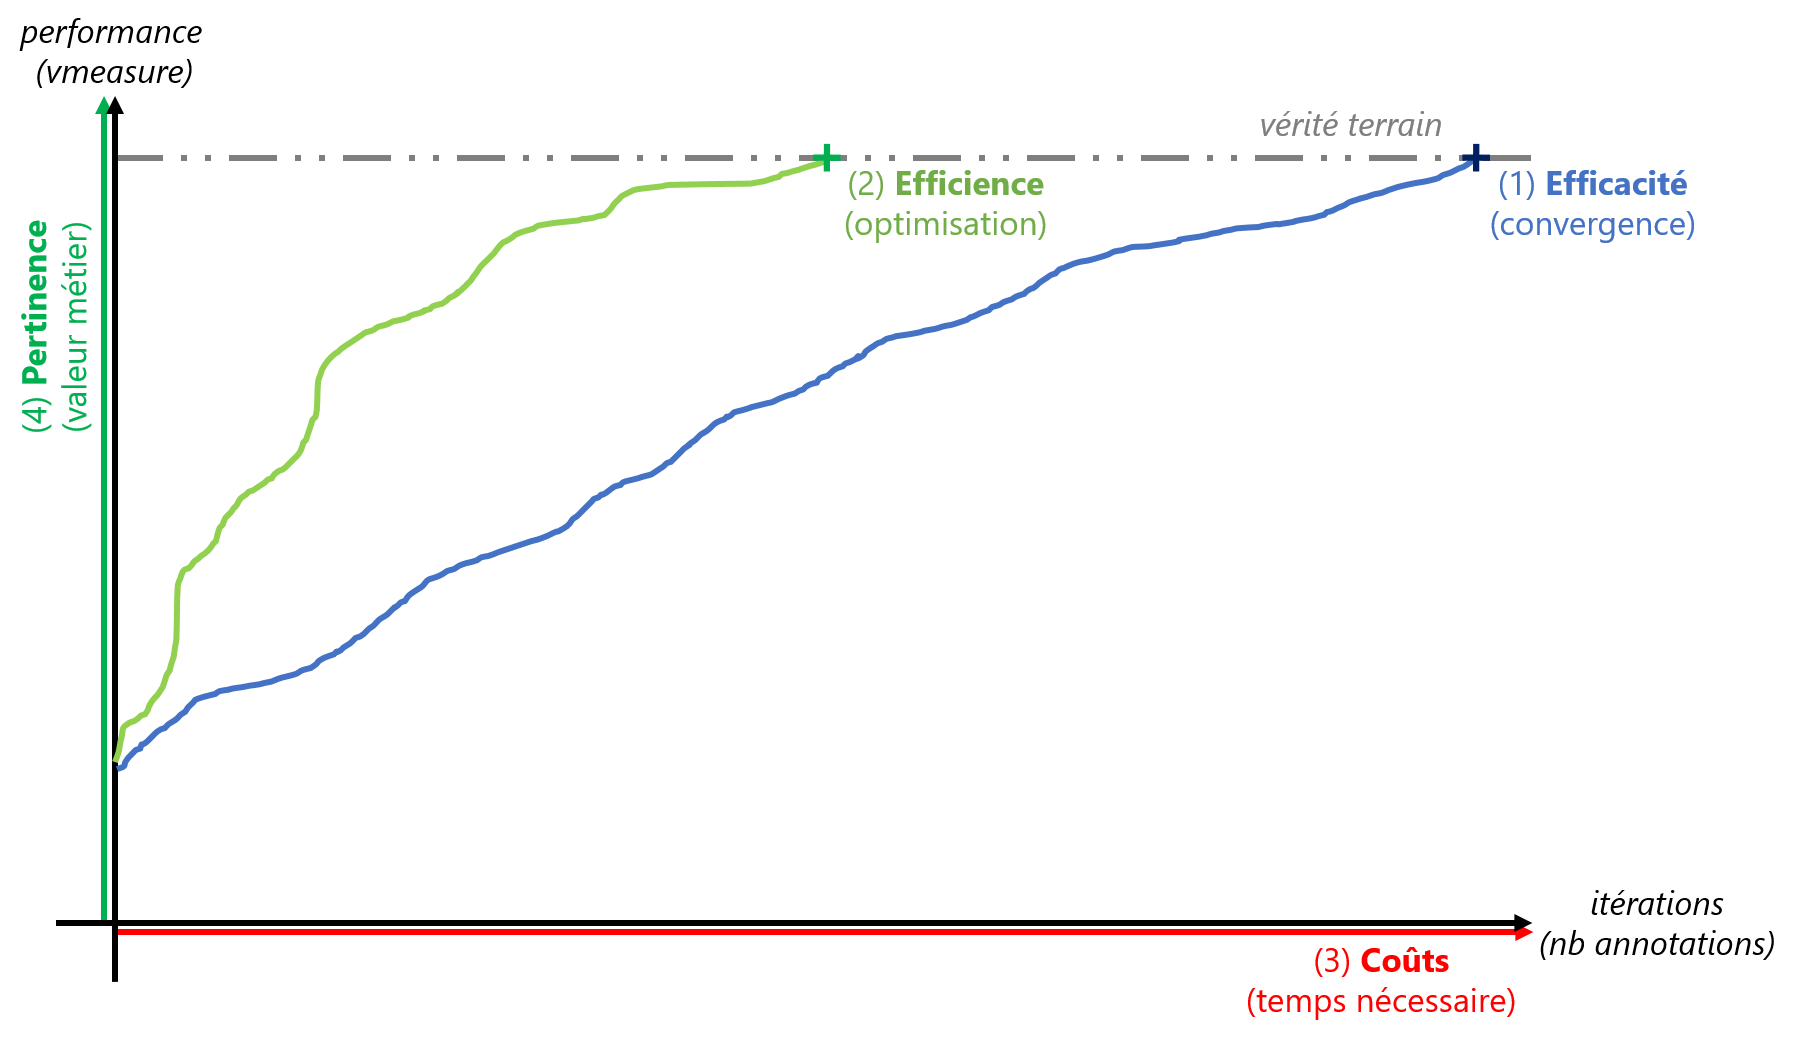
\includegraphics[width=0.8\textwidth]{figures/hypotheses-04-pertinence}
			\caption{Illustration des études réalisées sur le \textit{clustering} interactif (\textit{étape 4/6}) en schématisant l'évolution de la performance (\textit{accord avec la vérité terrain calculé en v-measure}) d'une base d'apprentissage en cours de construction en fonction du nombre d'itérations de la méthode (\textit{nombre d'annotations par un expert métier}).}
			\label{figure:4.4-HYPOTHESE-PERTINENCE}
		\end{figure}

	\end{tcolorbox}
	
	%%%
	%%% Subsection 4.4.1: Étude de la cohérence statistique de la base d'apprentissage en cours de construction
	%%%
	\subsection{Étude de la cohérence statistique de la base d'apprentissage en cours de construction}
	
		%%% Protocole expérimental.
		\subsubsection{Protocole expérimental}
			\todo[inline]{Description succincte du protocole expérimental dans l'encadré d'hypothèse ?}

		%%% Résultats
		\subsubsection{Résultats obtenus}
			%
			\begin{figure}[!htb]
				\centering
				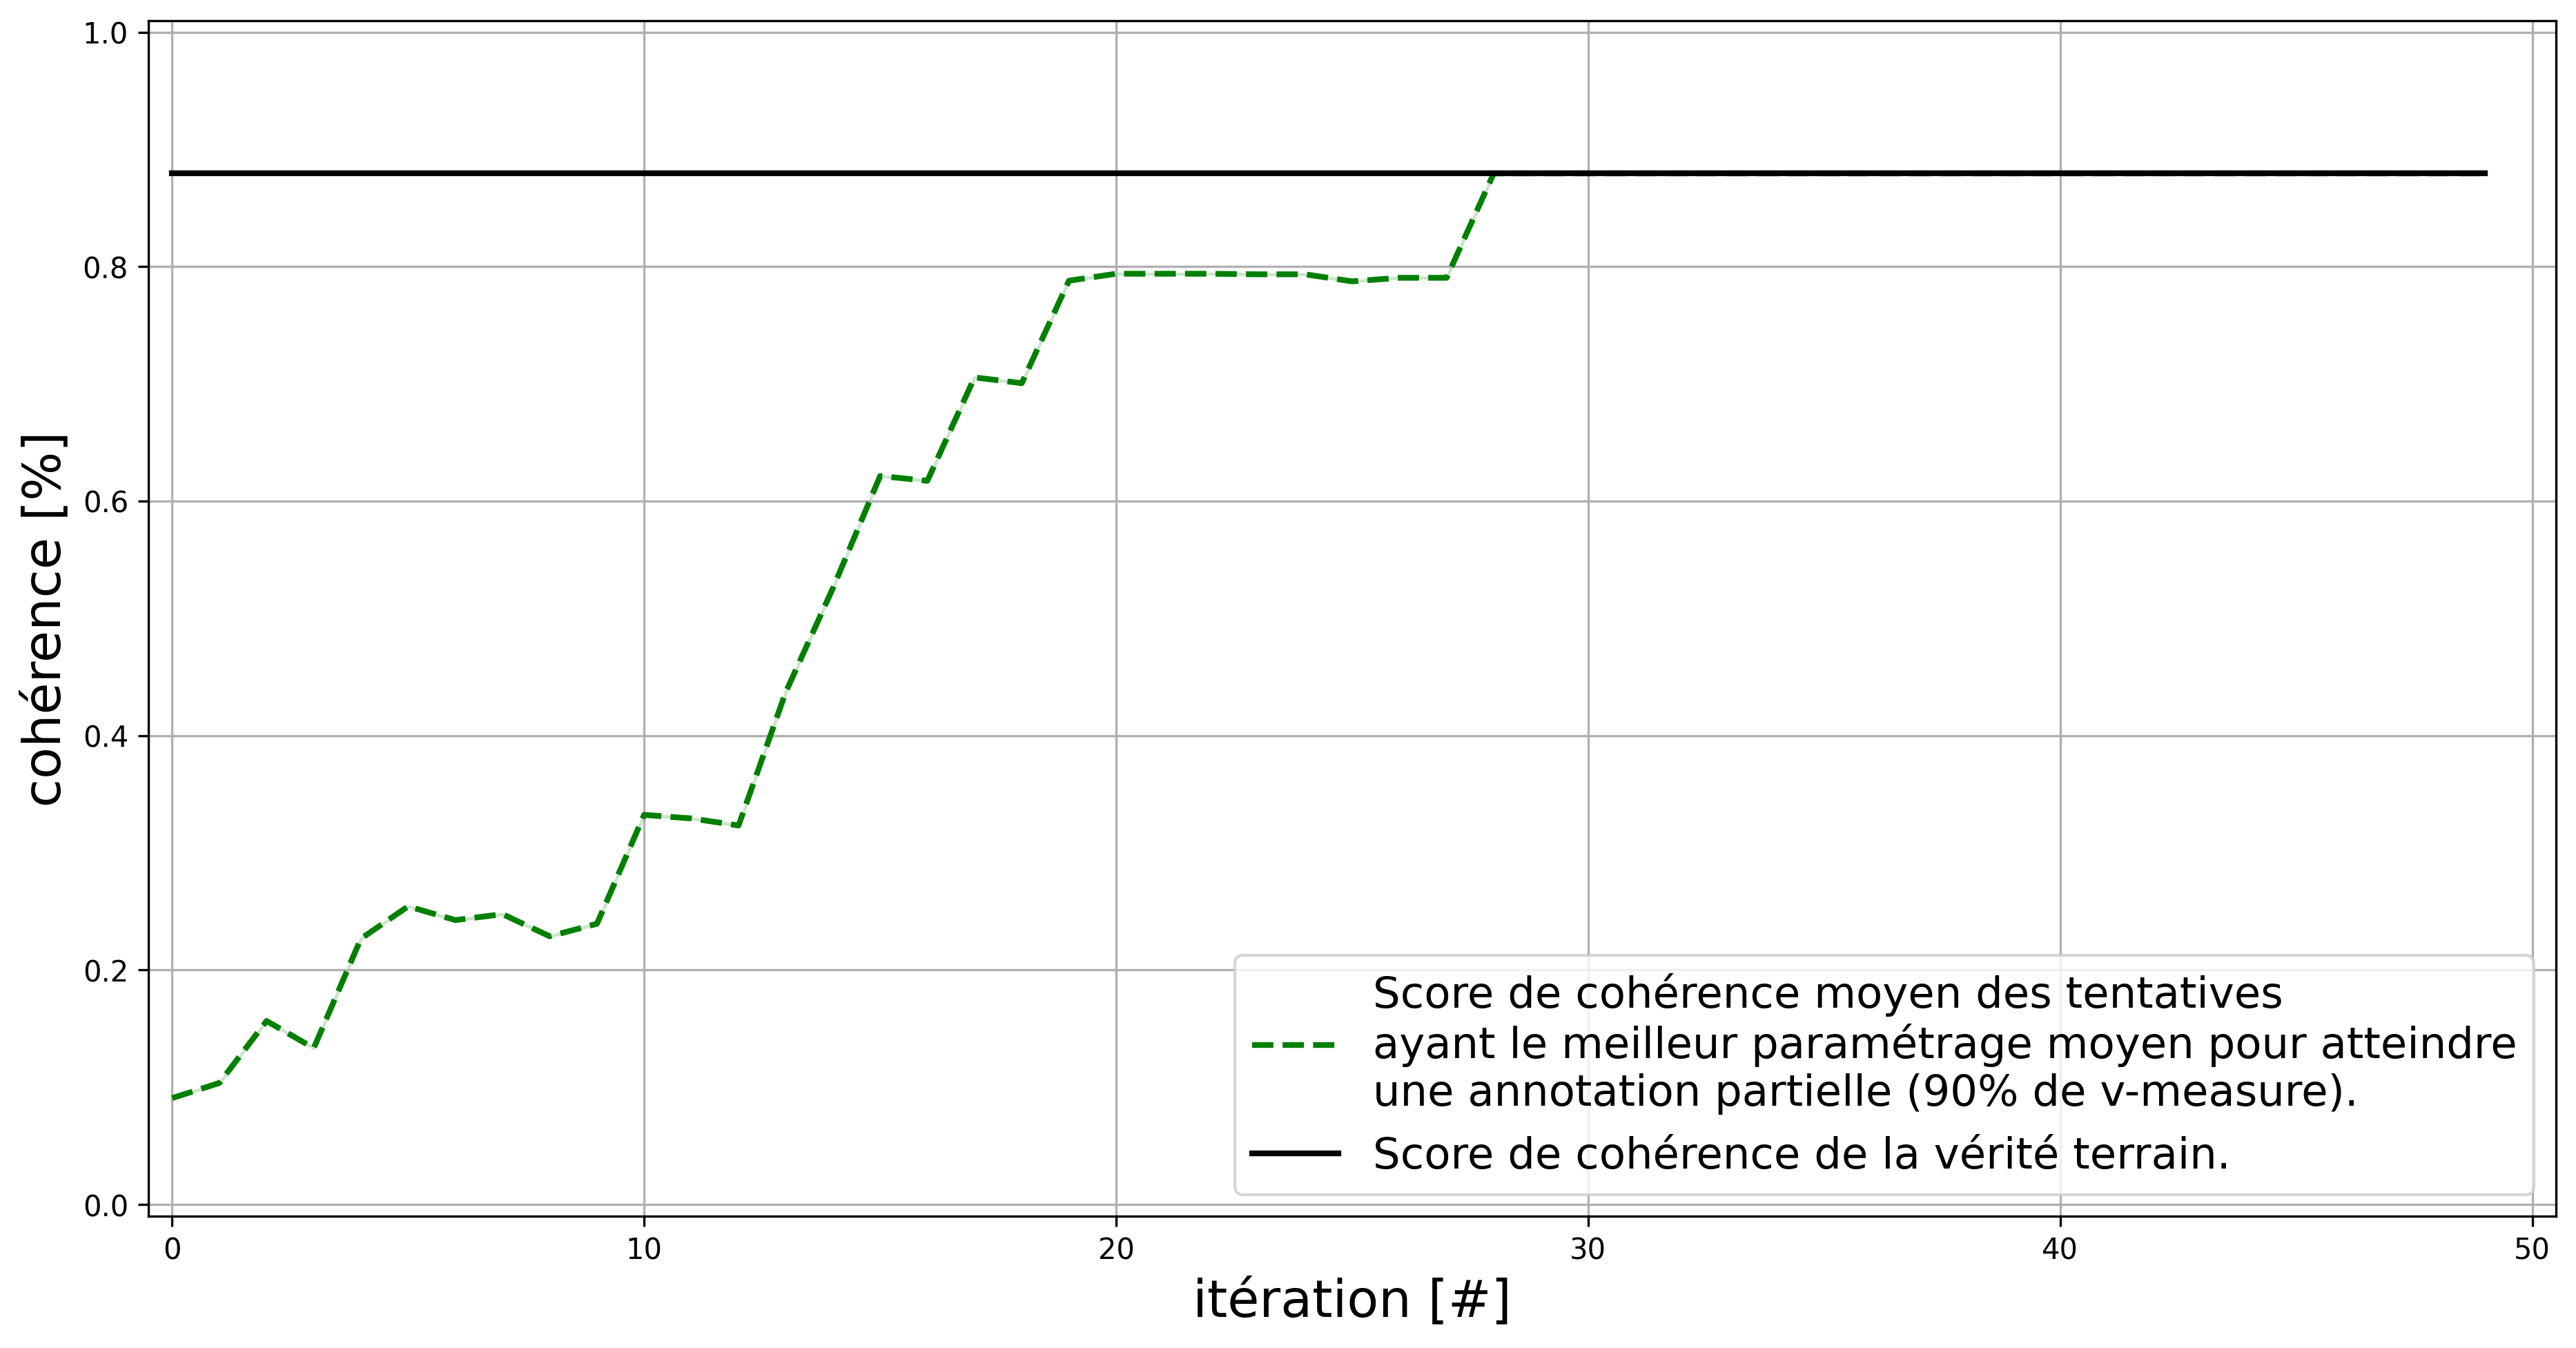
\includegraphics[width=0.8\textwidth]{figures/etude-pertinence-consistence-annotation-partielle}
				\caption{Évolution du score de cohérence moyen pour les tentatives ayant le meilleur paramétrage moyen pour atteindre une annotation partielle (\texttt{90}\% de \texttt{v-measure}).}
				\label{figure:4.3.1-ETUDE-PERTINENCE-CONHERENCE-ANNOTATION-PARTIELLE}
			\end{figure}

		%%% Discussion
		\subsubsection{Discussion}
	
	%%%
	%%% Subsection 4.4.2: Étude de la pertinence sémentique de la base d'apprentissage en cours de construction
	%%%
	\subsection{Étude de la pertinence sémantique de la base d'apprentissage en cours de construction}
	
		%%% Protocole expérimental.
		\subsubsection{Protocole expérimental}
			\todo[inline]{Description succincte du protocole expérimental dans l'encadré d'hypothèse ?}

		%%% Résultats
		\subsubsection{Résultats obtenus}

		%%% Discussion
		\subsubsection{Discussion}